\documentclass{article}

\usepackage[left=2cm,right=2cm,top=2cm,bottom=2cm]{geometry} 

\usepackage[utf8]{inputenc}   % otra alternativa para los caracteres acentuados y la "ñ"
\usepackage[           spanish % para poder usar el español
                      ,es-tabla % para los captions de las tablas
                       ]{babel}   
\decimalpoint %para usar el punto decimal en vez de coma para los números con decimales

%\usepackage{beton}
%\usepackage[T1]{fontenc}

\usepackage{parskip}
\usepackage{xcolor}

\usepackage{caption}

\usepackage{enumerate} % paquete para poder personalizar fácilmente la apariencia de las listas enumerativas

\usepackage{graphicx} % figuras
\usepackage{subfigure} % subfiguras

\usepackage{amsfonts}
\usepackage{amsmath}

\usepackage{listings}
\lstset
{ %Formatting for code in appendix
    language=python,
    basicstyle=\footnotesize,
    stepnumber=1,
    showstringspaces=false,
    tabsize=1,
    breaklines=true,
    breakatwhitespace=false,
}

\definecolor{gris}{RGB}{220,220,220}
	
\usepackage{float} % para controlar la situación de los entornos flotantes

\restylefloat{figure}
\restylefloat{table} 
\setlength{\parindent}{0mm}


\usepackage[bookmarks=true,
            bookmarksnumbered=false, % true means bookmarks in 
                                     % left window are numbered
            bookmarksopen=false,     % true means only level 1
                                     % are displayed.
            colorlinks=true,
            allcolors=blue,
            urlcolor=blue]{hyperref}
\definecolor{webblue}{rgb}{0, 0, 0.5}  % less intense blue

\begin{document}
\begin{center}
\vspace*{8cm}
{\Huge \textbf{Segmentación}}
\end{center}
\newpage
\tableofcontents
\newpage

\section{Introducción}

En esta práctica emplearemos técnicas de aprendizaje no supervisado,
como es el clustering, para realizar un análisis relacional mediante
segmentación.

Nuestro dataset consta de todos los accidentes ocurridos en España
durante el año 2013. Los datos están publicados por la
\href{https://sedeapl.dgt.gob.es/WEB_IEST_CONSULTA/subcategoria.faces}{DGT}. Disponemos
de datos de 89519 accidentes, y 32 variables que miden circunstancias
en las que ocurre cada accidente (día, hora, visibilidad, superficie
de la calzada, factores atmosféricos, zona \ldots), el tipo (alcance,
choque frontal, choque lateral, atropello a peatón o animal, colisión
con obstáculo \ldots) y la gravedad (número de heridos leves y graves y
número de muertos).

Los algoritmos de clustering que utilizaremos son:
\begin{itemize}
\item \href{https://en.wikipedia.org/wiki/K-means_clustering}{\textbf{K-means:}} Un algoritmo iterativo basado en
  particionamiento. Es relativamente eficiente ($O(tkn)$ donde $n$ es
  el número de datos, $k$ el de clústers y $t$ el de iteraciones) y
  suele alcanzar óptimos locales bastante buenos. Por otra parte, sólo
  trabaja bien cuando los datos son numéricos, necesita prefijar el
  número de clusters, sólo encuentra clusters esféricos y no lidia
  bien con datos ruidosos y outliers.

\item
  \href{https://en.wikipedia.org/wiki/DBSCAN}{\textbf{DBSCAN:}}
  También basado en particionamiento. No necesita a priori el número
  de clusters, en su lugar requiere el radio máximo de cada clúster y
  el tamaño mínimo de los mismos. También es capaz de encontrar
  clusters con distintas formas y es robusto a datos ruidosos y
  outliers.

\item \href{https://en.wikipedia.org/wiki/Ward%27s_method}
    {\textbf{Ward:}} Es un método aglomerativo, es decir, parte de un
    clúster para cada elemento y fusiona los clusters que generen en
    el agrupamiento con mínima varianza. Necesita el número de clúster
    o una distancia límite a partir de la cual no fusiona dos
    clusters.
\end{itemize}

Para estimar los hiperparámetros de los algoritmos atenderemos a dos
métricas para interpretar la bondad de un agrupamiento:

\begin{itemize}
\item \href{https://en.wikipedia.org/wiki/Silhouette_%28clustering%29}
    {\textbf{Coeficiente silhouette:}} Compara la similitud de de los
    objetos de un mismo cluster (cohesión) con los de otros clusters
    (separación). Para cada elemento $i$, se calcula $a(i)$ como la
    distancia media entre $i$ y el resto de elementos del cluster,
    mientras que que $b(i)$ representa el mínimo de las distancias
    entre $i$ y cada cluster distinto del suyo (la distancia de $i$ a
    un cluster se calcula como la media de las distancias de $i$ a
    cada elemento del cluster). Tomando
    \[s(i)=\frac{b(i)-a(i)}{\max{a(i),b(i)}}\] se tiene
    $s(i)\in[-1,1]$. Si $s(i)$ es negativo ($b(i)<a(i)$), claramente
    el elemento $i$ pertenece al cluster equivocado (está más cerca de
    un cluster distinto al suyo); si $s(i)$ está cerca de 1, significa
    que $i$ está mucho más cerca de los elementos de su cluster que
    del resto de clusters. El coeficiente silhoutte se calcula como la
    media de los $s(i)$ para todos los ejemplos $i$. Usualmente se
    encuentra entre 0 y 1.

  \item
    \href{https://www.tandfonline.com/doi/pdf/10.1080/03610927408827101?needAccess=true}{\textbf{Razón
        de Calinski-Harabasz:}} Razón entre la dispersión
    intra-clusters (dentro de cada cluster) cantidad que y la
    dispersión inter-clusters (entre clusters). Su cálculo es más
    complejo que el anterior y su valor no está entre 0 y 1, en
    nuestro caso toma valores del orden de miles.
  \end{itemize}

  Otro factor muy importante a tener en cuanta será el número de
  clusters generados, ya un elevado número de clusters dificulta las
  tareas de interpretación y análisis de los resultados. El hecho de
  generar un número excesivo de clusters con el fin de maximizar las
  métricas al precio de dificultar el análisis y la interpretabilidad
  sería el equivalente a lo que en aprendizaje supervisado conocíamos
  como sobreajuste, podemos llamarle también de ese modo.

  Debido al elevado número de datos, los algoritmos de clustering (que
  suelen presentar un elevado orden de complejidad) podrían tardar un
  tiempo excesivo en ejecutarse, por lo que realizaremos dos casos de
  estudio en cada uno de los cuales seleccionaremos un subconjunto de
  las instancias. Para cada caso de estudio, restringiremos el número
  de datos fijando los valores de una o más variables de carácter
  circunstancial o de tipo, y realizaremos el agrupamiento basándonos
  en las variables que miden la gravedad de los accidentes, pues son
  numéricas y nos evitan problemas como la dificultad de K-means para
  trabajar con variables nominales.

  Existe una amplia variedad de casos de estudio con sentido e interés
  que podríamos analizar: accidentes bajo condiciones climatológicas
  adversas, en zonas urbanas, atropellos, etc. Nosotros analizaremos
  los accidentes en condiciones óptimas para la conducción y los
  accidentes que ocurren a altas horas de la madrugada.

\section{Casos de estudio}
\section{Caso de estudio 1: Análisis de los accidentes en condiciones óptimas para la conducción}

El primer caso de estudio seleccionaremos los accidentes que ocurren
en condiciones óptimas para la conducción. Estos accidentes pueden
ocurrir bien por factor vehículo o bien por factor humano, ya que
eliminaremos el factor vía seleccionando ejemplos de accidentes que
ocurren en calzadas secas y limpias. No disponemos de datos relativos
al factor vehículo, pero dentro del factor humano, eliminaremos
también las condiciones que favorecen los errores humanos como la
falta de luminosidad, visibilidad o la circulación densa. Teniendo en
cuenta que el factor vehículo es causa de un porcentaje relativamente
bajo de accidentes (menos del 10\%), principalmente tenemos accidentes
debidos al factor humano que han ocurrido en condiciones óptimas para
la conducción: buen tiempo, buena visibilidad, calzada limpia y seca,
tráfico fluido, etc. Es decir, accidentes debidos a factor humano que
se podrían haber evitado. Aquí radica el interés de este caso de
estudio.

En concreto, estos son los valores que fijamos para las variables:

\begin{verbatim}
LUMINOSIDAD=='NOCHE: ILUMINACIÓN SUFICIENTE' | LUMINOSIDAD=='PLENO DÍA'
DENSIDAD_CIRCULACION=='FLUIDA'
DIASEMANA==6
OTRA_CIRCUNSTANCIA=='NINGUNA'
FACTORES_ATMOSFERICOS=='BUEN TIEMPO'
MEDIDAS_ESPECIALES=='NINGUNA MEDIDA'
SUPERFICIE_CALZADA=='SECA Y LIMPIA'
VISIBILIDAD_RESTRINGIDA=='SIN RESTRICCIÓN'
\end{verbatim}

Con \texttt{OTRA\_CIRCUNSTANCIA=='NINGUNA'} descartamos accidentes
ocurridos con obras, inundaciones, baches, badenes, cambios de
rasante, estrechamientos, pasos a nivel y demás circunstancias que
podrían dificultar la conducción. Con
\texttt{MEDIDAS\_ESPECIALES=='NINGUNA MEDIDA'} descartamos accidentes
ocurridos en carriles reversibles o con habilitación del arcén, que
podríamos considerar fuera de la conducción ``normal''.

Además, para quedarnos con menos datos nos restringimos a los
accidentes ocurridos en sábado con \texttt{DIASEMANA==6}. Los días del
lunes al jueves son más propensos a presentar accidentes con una sola
víctima (como apreciamos en la Figura \ref{fig:diasemana}), esto ocurre
porque va mucha más gente a trabajar, mientras que en fin de semana es
más usual que viajen varias personas en el coche. Así que elegimos
este día para obtener un mayor número de accidentes con múltiples
víctimas. El hecho de que viajen más personas en el coche a parte del
conductor, por una parte puede aumentar la responsabilidad y por otra
puede aumentar las distracciones o crear una falsa sensación de
confianza. Esto hace los accidentes ocurridos en fin de semana más
interesantes, en mi opinión. Motivo por el cuál elegimos un día del
fin de semana.

\begin{figure}[H]
  \centering
  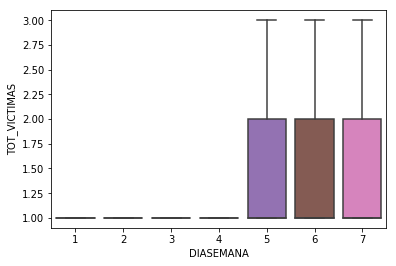
\includegraphics[width=97mm]{figures/accidentes/diasemana}
  \caption{De lunes a jueves la mayoría de accidentes ocasionan una
    sola víctima (considera los accidentes con más víctimas como
    outliers). En fin de semana hay más accidentes con múltiples
    víctimas.}
  \label{fig:diasemana}
\end{figure}

Fijando estos valores, nos quedamos con 4143 instancias, por lo que
nuestros algoritmos se ejecutarán bastante rápido.

\subsection{Algoritmos de clustering y resultados}

\subsubsection{K-means}

\href{https://scikit-learn.org/stable/modules/generated/sklearn.cluster.KMeans.html}{\textbf{K-means:}}

\subsubsection{Ward}

\subsubsection{Comparación}

\href{https://scikit-learn.org/stable/modules/generated/sklearn.cluster.AgglomerativeClustering.html}{implementacion ward}

\subsection{Interpretación de la segmentación}

\section{Caso de estudio 2: Análisis de los accidentes a altas horas de la madrugada}

\subsection{Algoritmos de clustering y resultados}

\subsubsection{K-means}

\href{https://scikit-learn.org/stable/modules/generated/sklearn.cluster.DBSCAN.html}{\textbf{DBSCAN:}}

\subsubsection{BDSCAN}

\subsubsection{Comparación}

\subsection{Interpretación de la segmentación}

\end{document}
